\begin{XeClass}{FSInputChecker}
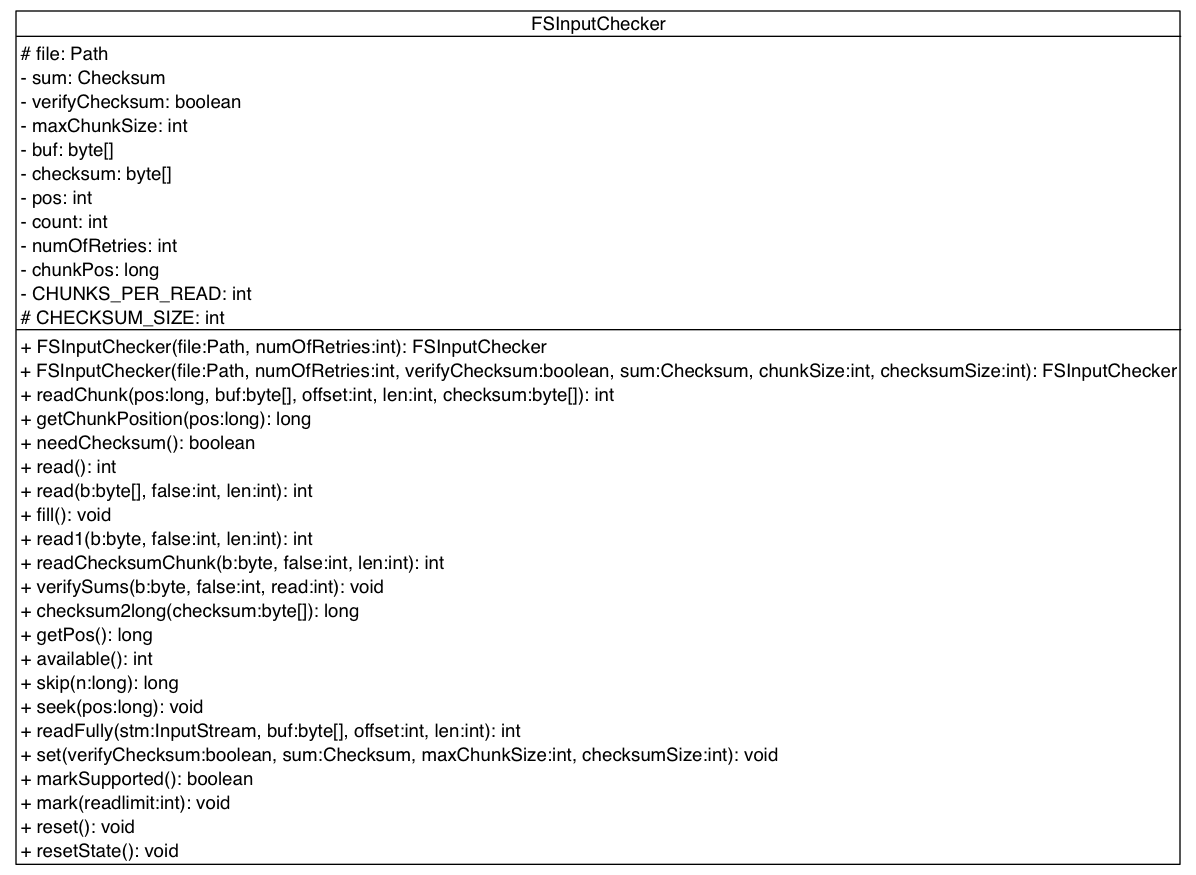
\includegraphics[width=10cm]{cdig/FSInputChecker.png}
    
    \begin{XeMethod}{\XeProtected}{FSInputChecker}{FSInputChecker}
         
 构造函数

    \end{XeMethod}

    \begin{XeMethod}{\XeProtected}{FSInputChecker}{FSInputChecker}
         
 构造函数

    \end{XeMethod}

    \begin{XeMethod}{\XeAbstract \\ \XeProtected}{int}{readChunk}
         
 从文件中读取数据和校验和,将数据放入buf,将校验和放入checksum。
 如果len不是ChunkSize的整数倍,那么将会读取少于len个字节,以保证
 读取的数据量为ChunkSize的整数倍。
 如果校验和功能被禁用,则在checksum位置传入null,并且在读取时不会
 因为len不是ChunkSize的整数倍而导致读取字节数小于len。

    \end{XeMethod}

    \begin{XeMethod}{\XeAbstract \\ \XeProtected}{long}{getChunkPosition}
         
 返回pos位置所在的Chunk

    \end{XeMethod}

    \begin{XeMethod}{\XeProtected \\ \XeSync}{boolean}{needChecksum}
         
 返回是否需要校验

    \end{XeMethod}

    \begin{XeMethod}{\XePublic \\ \XeSync}{int}{read}
         
 从当前缓冲区读取一个字节

    \end{XeMethod}

    \begin{XeMethod}{\XePublic \\ \XeSync}{int}{read}
         
 读取len个字节到字节数组b的偏移量off处,读取的数据都经过校验。
 此方法会尝试不断读取,知道读取到len个字节,直到EOF或者IOException

    \end{XeMethod}

    \begin{XeMethod}{\XePrivate}{void}{fill}
         
 向buf中填充一个经过校验的chunk

    \end{XeMethod}

    \begin{XeMethod}{\XePrivate}{int}{read1}
         
 读取len个字节到字节数组b的偏移量off处,如果len超出了Chunk的大小
 则会先向缓冲区中填入一个Chunk,再从buf复制到b中。

    \end{XeMethod}

    \begin{XeMethod}{\XePrivate}{int}{readChecksumChunk}
         
 读取一个或多个经过校验和检查的Chunk到b指定的字节数组的偏移量offset处,
 这个方法保证所有读取到的数据都是经过校验。

    \end{XeMethod}

    \begin{XeMethod}{\XePrivate}{void}{verifySums}
         
 计算字节数组b中的要进行校验的数据的校验和,并与checksum中的,即当前读取的
 chunk的校验和进行比较

    \end{XeMethod}

    \begin{XeMethod}{\XePublic}{long}{checksum2long}
         
 将一个checksum转换为一个long数字

    \end{XeMethod}

    \begin{XeMethod}{\XePublic \\ \XeSync}{long}{getPos}
         
 返回当前文件的读取位置

    \end{XeMethod}

    \begin{XeMethod}{\XePublic \\ \XeSync}{int}{available}
         
 返回当前缓冲区中尚未读取的字节。

    \end{XeMethod}

    \begin{XeMethod}{\XePublic \\ \XeSync}{long}{skip}
         
 在输入流中跳过并忽略n个字节,如果n是负数,则不会跳过任何字节。

    \end{XeMethod}

    \begin{XeMethod}{\XePublic \\ \XeSync}{void}{seek}
         
 移动读取位置到pos,下一次read将会从pos位置读取。

    \end{XeMethod}

    \begin{XeMethod}{\XeProtected}{int}{readFully}
         
 A utility function that tries to read up to \emph{len} bytes from
 \emph{stm}
 一个静态工具类,从\emph{stm</code>中读取<code>len}个字节,放入buf
 中的offset位置。

    \end{XeMethod}

    \begin{XeMethod}{\XeFinal \\ \XeProtected \\ \XeSync}{void}{set}
         
 设置校验和相关参数

    \end{XeMethod}

    \begin{XeMethod}{\XeFinal \\ \XePublic}{boolean}{markSupported}
         
 不支持mark

    \end{XeMethod}

    \begin{XeMethod}{\XeFinal \\ \XePublic}{void}{mark}
         
 不支持mark

    \end{XeMethod}

    \begin{XeMethod}{\XeFinal \\ \XePublic}{void}{reset}
         
 不支持reset

    \end{XeMethod}

    \begin{XeMethod}{\XePrivate}{void}{resetState}
         
 重置FSInputChecker的state

    \end{XeMethod}

\end{XeClass}
